\documentclass[runningheads]{llncs}

\usepackage{booktabs}
\usepackage{microtype}
\usepackage{xcolor}
\usepackage{hyperref}
\usepackage{xspace}
\usepackage{amsmath}
\usepackage{graphicx}
\usepackage{tikz}
\usetikzlibrary{arrows.meta,positioning,fit}

\hypersetup{colorlinks=true,linkcolor=blue,citecolor=blue,urlcolor=blue}
\newcommand{\system}{\textsc{Skill Runtime Intelligence}\xspace}
\newcommand{\panorama}{\textsc{Run Panorama}\xspace}
\newcommand{\observed}{\textsc{Observed}\xspace}
\newcommand{\derived}{\textsc{Derived}\xspace}
\newcommand{\inferred}{\textsc{Inferred}\xspace}
\newcommand{\experimental}{\textsc{Experimental}\xspace}

\title{Evidence-Calibrated Runtime Reconstruction for Agent Skills Across
Heterogeneous Coding Agents}
\titlerunning{Evidence-Calibrated Runtime Reconstruction for Agent Skills}
\author{Author Information Required}
\authorrunning{Author Information Required}
\institute{Affiliation and email required before submission}

% LNCS is an A4 proceedings format. This driver hint keeps XeTeX/Tectonic's
% PDF media box aligned with the class layout; it is ignored by other drivers.
\special{papersize=210mm,297mm}

\begin{document}
\maketitle

\begin{abstract}
Agent Skills package reusable instructions, scripts, references, and assets for
tool-using language-model agents.  Their progressive loading protocol creates
failure boundaries that are poorly represented by session-, model-, or
tool-centric traces: a Skill may be discovered but not activated, activated
without loading its instructions, or appear successful without an independently
verified outcome.  We present \system, a local-first, read-only runtime evidence
system that reconstructs a Skill-specific lifecycle across heterogeneous agent
harnesses.  Its central abstraction, the \panorama, separates immutable source
events, deterministic relations, uncertain diagnoses, and controlled
experimental outcomes using four evidence grades.

We evaluate the design with six frozen repository profiles,
three installed coding agents, and seven clean or fault-injected conditions.
All 126 executions preserve their source worktrees and correlate to exactly one
source session, yet current adapters expose sharply different semantics: one
emits no Skill runs, one reconstructs all runs but no failure-like events, and
one emits failure-like events in all 24 failure-condition sessions and all six
clean sessions. A privacy-safe diagnostic study instantiates seven repeated
condition templates. Semantic aliases and Panorama both localize the six
non-clean boundaries, while exact/status behavior varies by template; both Raw
views emit a failure status on all 18 clean instantiations, whereas Panorama
does not. A deterministic lifecycle graph conforms to all 126 known-rule
contracts. A second model completes only 228/378 requested calls. These
controlled mechanism observations show that event presence is not boundary
fidelity, composite exact scores can conceal distinct error types, and model
explanations should not overwrite deterministic runtime facts.
\end{abstract}

\keywords{Agent Skills \and runtime observability \and evidence provenance
\and coding agents \and empirical software engineering}

\section{Introduction}

Language-model agents increasingly acquire reusable capabilities through
\emph{Skills}: directories containing declarative metadata and optional
scripts, references, and assets.

The specification uses progressive disclosure: lightweight metadata may
be visible before full instructions or resources are loaded
\cite{agent-skills-spec}.  This improves modularity but creates a new operational
question: \emph{did the Skill actually run as intended?}

The final answer is insufficient evidence.  A plausible answer may follow a
missed activation, a missing reference, a failed command, or an unverified
artifact.  Conversely, missing telemetry does not prove that a lifecycle step
failed.  Existing agent evaluation commonly measures task success or trajectory
quality \cite{swebench,agentdiagnose}; general tracing standards model
agent and tool spans \cite{otel-genai}, but do not make a dynamically loaded
Skill occurrence, its resource boundary, or its evidence grade the primary
entity.  The operational gap is therefore not simply ``more tracing.''  It is
the reconstruction of a portable Skill lifecycle from incomplete,
harness-specific evidence without inventing observations.

We introduce \system, a passive runtime evidence architecture for Agent Skills.
It observes existing agent workflows rather than proxying model requests or
orchestrating the agent.  Versioned adapters retain raw source events and map
them into a common event model.  A deterministic evidence graph reconstructs
Skill occurrences and lifecycle relations.  Diagnoses state both their
evidential basis and their causal scope.  Model-based analysis is restricted to
an \inferred layer and cannot promote or overwrite deterministic facts.

Our study asks four research questions:

\begin{description}
  \item[RQ1:] How faithfully can heterogeneous agent telemetry reconstruct a
  Skill lifecycle and its first divergent boundary?
  \item[RQ2:] How does a normalized Panorama change exact diagnosis, boundary
  localization, status, and evidence entailment relative to raw events, and
  when are deterministic or model-assisted diagnoses justified?
  \item[RQ3:] Can collection remain read-only, local, silent, and low-overhead?
  \item[RQ4:] What controlled mechanism coverage is observed across frozen
  repository profiles, agents, environments, and model backends?
\end{description}

This paper makes four contributions:

\begin{enumerate}
  \item A Skill-specific runtime event model and lifecycle that distinguish
  occurrence from relationship attribution.
  \item A four-grade evidence contract---\observed, \derived, \inferred, and
  \experimental---with explicit causal-scope restrictions.
  \item A local-first system with versioned adapters, immutable raw evidence,
  deterministic reconstruction, and non-authoritative model assistance.
  \item A reproducible controlled benchmark over six frozen three-file
  repository profiles, three installed agents, seven condition families, two model backends, and
  independent nonce-bound outcome verification, including paired diagnostic
  transitions and family-stratified failure analysis.
\end{enumerate}

The study supports claims about controlled reconstruction and evidence
architecture.  It does not estimate natural incident prevalence, human
usability, causal Skill effectiveness, or unconstrained production diagnosis
accuracy.

\section{Problem and Design Requirements}

\subsection{The Skill lifecycle}

We represent one attempted Skill execution as the ordered lifecycle

\begin{center}
\small
Request $\rightarrow$ Discovery $\rightarrow$ Activation $\rightarrow$
Instructions $\rightarrow$ Resources $\rightarrow$ Execution $\rightarrow$
Artifacts $\rightarrow$ Outcome.
\end{center}

The stages are logical boundaries, not a requirement that every harness emit a
span for every stage.  A resource access can be directly observed while its
membership in a particular Skill occurrence is only deterministically derived.
An agent may report success while the outcome remains unverified.  This
separation prevents two common errors: treating absence of telemetry as a
failure, and treating an agent assertion as an independently verified result.

\subsection{Requirements}

Our design follows six requirements.

\paragraph{R1: Observation without takeover.}
The system must not proxy model requests, own the agent loop, or block actions
by default.  Collection should be compatible with normal agent use.

\paragraph{R2: Source preservation.}
Raw records are immutable and remain separately addressable.  Normalization
cannot erase source identity, and multiple physical streams with the same
upstream session identifier cannot overwrite one another.

\paragraph{R3: Epistemic separation.}
Facts directly supplied by a source, deterministic transformations, uncertain
analysis, and controlled effect estimates must not share one undifferentiated
confidence field.  This follows the broader provenance principle that entities,
activities, and derivations should retain explicit relations
\cite{w3c-prov-dm}.

\paragraph{R4: Versioned capability.}
Adapters are measurement instruments whose schemas and coverage change with
agent versions.  Every normalized record binds agent, agent version, adapter
version, and source format.  Unsupported fields remain unknown.

\paragraph{R5: Privacy by minimization.}
Prompts, code, paths, credentials, and raw payloads are not required for most
lifecycle diagnoses.  The default store is local, and exported research views
contain only the minimum ordered states and opaque evidence identifiers.

\paragraph{R6: Causal restraint.}
A single run may establish that an event occurred or that a verifier passed; it
cannot establish that the Skill caused the outcome.  Skill-effect claims require
controlled repeated trials and are labeled \experimental.

\section{System Architecture}

\begin{figure}[t]
\centering
\resizebox{\textwidth}{!}{%
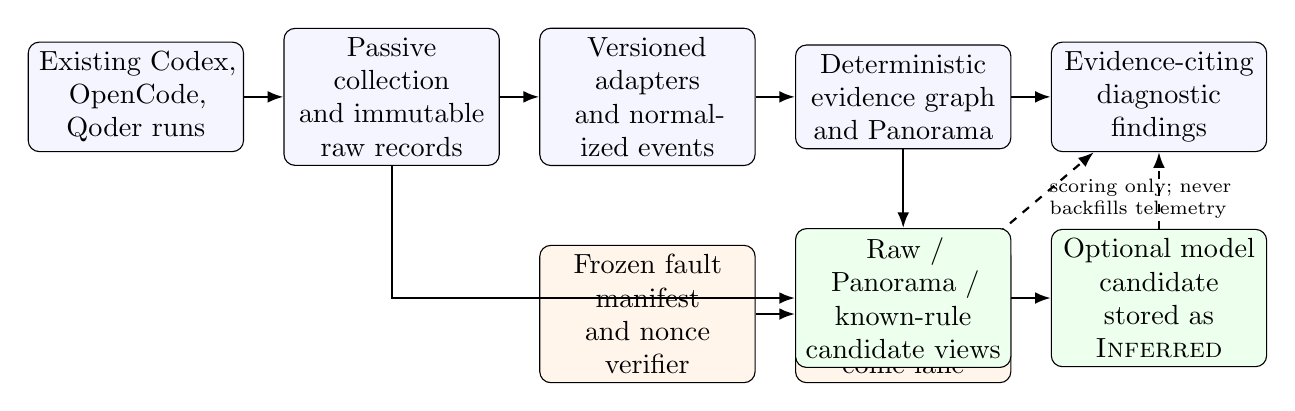
\begin{tikzpicture}[
  node distance=5mm and 5mm,
  box/.style={draw,rounded corners,align=center,minimum height=8mm,
    text width=25mm,fill=blue!4},
  oracle/.style={box,fill=orange!8},
  model/.style={box,fill=green!7},
  arr/.style={-{Latex[length=2mm]},thick},
  dasharr/.style={arr,dashed}
]
\node[box] (agents) {Existing Codex,\\OpenCode, Qoder runs};
\node[box,right=of agents] (raw) {Passive collection\\and immutable raw records};
\node[box,right=of raw] (adapter) {Versioned adapters\\and normalized events};
\node[box,right=of adapter] (graph) {Deterministic evidence graph\\and Panorama};
\node[box,right=of graph] (finding) {Evidence-citing\\diagnostic findings};
\draw[arr] (agents)--(raw);
\draw[arr] (raw)--(adapter);
\draw[arr] (adapter)--(graph);
\draw[arr] (graph)--(finding);

\node[oracle,below=10mm of adapter] (manifest) {Frozen fault manifest\\and nonce verifier};
\node[oracle,right=of manifest] (gold) {Gold boundary/status\\and outcome lane};
\draw[arr] (manifest)--(gold);
\draw[dasharr] (gold)--node[right,align=left,font=\scriptsize]
  {scoring only; never\\backfills telemetry} (finding);

\node[model,below=10mm of graph] (views) {Raw / Panorama /\\known-rule candidate views};
\node[model,right=of views] (llm) {Optional model candidate\\stored as \inferred};
\draw[arr] (raw.south)|-(views.west);
\draw[arr] (graph.south)--(views.north);
\draw[arr] (views)--(llm);
\draw[dasharr] (llm)--(finding);
\end{tikzpicture}}
\caption{Production data flow (top) and evaluation-only oracle lane (orange).
The controlled fault manifest supplies gold labels to the scorer, not observed
telemetry.  The deterministic graph is evaluated as known-rule contract
conformance; the optional model remains non-authoritative.}
\label{fig:architecture}
\end{figure}

\subsection{Data path}

\system has four layers:

\begin{enumerate}
  \item \textbf{Collectors} ingest official hooks, local transcripts, and
  read-only filesystem or process signals.
  \item \textbf{Versioned adapters} retain raw source records and emit a common
  event envelope with timestamp and source provenance.
  \item \textbf{The evidence engine} constructs sessions, turns, Skill runs,
  resources, tools, artifacts, outcomes, and typed relations.
  \item \textbf{The Panorama and diagnostics} expose the lifecycle, the first
  observable divergence, the supporting evidence, and unobservable boundaries.
\end{enumerate}

The architecture complements rather than replaces span-centric observability.
OpenTelemetry's generative-AI conventions describe agent invocation and tool
execution spans \cite{otel-genai}; \system adds a domain layer centered on a
versioned Skill definition and one occurrence of that definition.

\subsection{Event and identity model}

Each normalized event contains a locally unique identifier, event type,
occurrence and ingestion times, physical source session, optional turn and Skill
run identifiers, source locator, adapter identity, and evidence metadata.  The
event vocabulary covers session and turn state, Skill discovery and activation,
instruction and resource access, tool and subagent execution, workspace and
artifact activity, and reported, verified, or unknown outcomes.

Physical evidence streams and logical upstream session IDs are intentionally
separate.  A correlation key may join streams for analysis but never authorizes
destructive merging.  Similarly, an event's existence and the edge assigning it
to a Skill run are separate claims.  Exact path and identifier boundaries avoid
prefix collisions such as assigning \texttt{pdf-backup} activity to
\texttt{pdf}.

Stable identities combine adapter version, physical source-instance identity,
and explicit source event or call identifiers; timestamps alone never create
identity. Reconstruction applies fixed precedence: source parent/child ID,
explicit Skill attribution, active Skill scope, exact artifact path, temporal
adjacency, then model or heuristic suggestion. The first four may create
\derived edges. The last two remain uncertain and cannot replace a
higher-priority edge. Conflicting equal-priority relations are retained as
ambiguous rather than resolved by timestamp proximity.

The engine (1) appends the immutable raw record, (2) consults the
adapter-version capability declaration, (3) emits only supported normalized
fields, (4) attaches deterministic edges in precedence order, (5) traverses the
eight lifecycle stages, and (6) emits a finding only when an observed failure or
an evaluable expected signal establishes a boundary. An optional model runs
after this procedure. For example, a source \texttt{Skill} call is retained,
normalized to \texttt{skill.\allowbreak activated} as \observed, and connected to subsequent
tool activity by a separately graded \texttt{skill\_\allowbreak scope} edge; a model
explanation is stored in a different \inferred record. The implementation is
approximately 11.7k Python lines spanning versioned adapters, storage,
redaction, reconstruction, diagnostics, export, server, and local UI.

\subsection{Evidence grades and causal scope}

Table~\ref{tab:evidence} defines the evidence contract.  Grade is about how a
claim is known; causal scope is a separate authorization decision.  For example,
an independently verified subprocess failure is \observed or \derived evidence
of an outcome, but still does not establish a Skill-to-outcome causal effect.

\begin{table}[t]
\centering
\caption{Evidence grades. Cross-run causal effects require controlled trials.}
\label{tab:evidence}
\small
\begin{tabular}{p{0.18\columnwidth}p{0.70\columnwidth}}
\toprule
Grade & Meaning \\
\midrule
Observed & Directly present in a source record or external verifier. \\
Derived & Deterministic transformation or relation over observed records. \\
Inferred & Uncertain model or heuristic explanation; never promoted silently. \\
Experimental & Estimate from a declared controlled experiment. \\
\bottomrule
\end{tabular}
\end{table}

\subsection{Deterministic diagnosis graph}

The evidence engine maps each lifecycle stage to observed success, observed
failure, expected but not observed, unsupported, or not applicable.
Versioned rules traverse ordered stages and typed edges to produce a candidate
boundary and status.  Each finding cites the exact node or relation that entails
it.  Missing events only become a finding when the adapter capability and an
independent expectation make the absence evaluable.

Model analysis receives a minimized view and returns a structured candidate,
status, evidence IDs, and causal flag.  It is stored as \inferred.  A combined
graph-and-model condition may explain or rank deterministic candidates, but the
production contract does not allow it to overwrite a graph fact.  The
experiment deliberately permits that change so the risk is measurable.

\section{Evaluation Methodology}

\subsection{Experimental principles}

We preregister the condition matrix and gates in machine-readable manifests.
Source execution, telemetry reconstruction, agent response, and model diagnosis
are separate endpoints.  Failed gates and malformed outputs remain in the
reports; we do not silently retry them.  Repositories are read through frozen
Git objects, so pre-existing dirty files are provenance covariates but not
experimental inputs.  SHA-256 binds fixtures, probes, and reports.

Our methodology resembles executable repository benchmarks such as SWE-bench
\cite{swebench} in freezing code state and using an external oracle, but differs
in target: we measure Skill-lifecycle evidence rather than patch correctness.

\subsection{Multi-repository Agent benchmark}

We freeze three tracked files from each of six Git repository profiles: two Go
projects, two Python research projects, and two Agent Skill or specification
projects.  Each repository receives a repository-specific, read-only audit
Skill.  A deterministic probe operates on a temporary overlay and emits a
nonce-bound oracle record.  Source worktrees must remain byte-identical.

\begin{table}[t]
\centering
\caption{Frozen repository profiles. Revisions and selected files are bound by
the manifest; diversity is profile-level, not repository-scale.}
\label{tab:profiles}
\scriptsize
\begin{tabular}{@{}lll@{}}
\toprule
Profile & Type & Frozen files (three each) \\
\midrule
tinylru & Go cache & \texttt{go.mod}, implementation, test \\
rapid-tele & Go telemetry & README, \texttt{go.mod}, agent \\
llm-mi & Python research & packaging, config, activation \\
llm-mech-int. & Python app & README, requirements, app \\
hello-skill & Spec workflow & constitution, shell helper, check \\
rapid-agent & Skill catalog & README, Skill, shell helper \\
\bottomrule
\end{tabular}
\end{table}

The benchmark crosses three installed coding-agent CLIs---Codex, OpenCode, and
Qoder---with seven conditions: clean, instruction failure, missing resource,
execution failure, artifact corruption, unverified outcome, and verifier
conflict.  This yields $6\times3\times7=126$ cells.  There is one execution per
cell; the experiment establishes mechanism coverage, not stochastic population
rates.  Per agent, the matrix contains 24 operational failure cells (four
failure boundaries across six repositories), six clean cells, and 12
outcome-evidence cells (unverified outcome and verifier conflict).  We report
these denominators separately because outcome-evidence conflicts are not native
execution failures.

We use two independent gates.  The \emph{integrity gate} requires every cell to
launch, preserve its workload, and correlate to exactly one collected source
session.  The stricter \emph{response gate} additionally requires the agent to
return the exact nonce-bound oracle JSON.  Reconstruction is scored separately
for Skill-run coverage, failure-like-event co-occurrence, clean
failure-like-event rate, and exact first-boundary localization.  The
co-occurrence metric does not attribute an arbitrary failed event to the
injected nonce or boundary.

Table~\ref{tab:agents} fixes the execution interfaces used in this study.  These
are adapter--version observations, not rankings of the underlying models or
products.

\begin{table}[t]
\centering
\caption{Installed agent interfaces used for the 126-cell benchmark.}
\label{tab:agents}
\small
\begin{tabular}{@{}llll@{}}
\toprule
CLI & Version & Model/mode & Environment \\
\midrule
Codex & 0.145.0 & \texttt{gpt-5.6-sol} & macOS arm64 \\
OpenCode & 1.18.5 & \texttt{deepseek-v4-flash-free} & macOS arm64 \\
Qoder & 1.1.10 & \texttt{performance} & macOS arm64 \\
\bottomrule
\end{tabular}
\end{table}

\subsection{Diagnostic utility study}

The 126 collected cases are transformed into a privacy-safe holdout that omits
raw content, paths, payloads, timestamps, and source session IDs.  Gold labels
come from the frozen fault manifest and deterministic probe, not a model or
human adjudicator.  The cases repeat seven semantic condition templates across
repositories and agents; they are paired cases, not 126 independent fault
families.  Raw and Panorama are programmatic views of the same controlled
execution.  We compare four primary views and one Qwen-only control:

\begin{enumerate}
  \item \textbf{Raw model}: ordinal native events with minimal structure;
  \item \textbf{Semantics-matched Raw}: every native and auxiliary record is
  retained while inline aliases expose Panorama-equivalent lifecycle, kind,
  status, and evidence-grade semantics;
  \item \textbf{Panorama model}: normalized lifecycle stages and evidence grades;
  \item \textbf{Known-rule graph}: deterministic typed-relation candidate;
  \item \textbf{Graph+Model}: the graph candidate plus a model explanation pass.
\end{enumerate}

For the primary model conditions, each case is evaluated in Raw, Panorama, and
Graph+Model views, or 378 calls per backend. The semantics-matched control adds
126 Qwen calls. Primary metrics are exact boundary-and-status diagnosis,
boundary accuracy, status accuracy, citation-ID validity, citation entailment,
causal safety, completion, and latency.  Citation entailment is stricter than
checking whether an identifier exists: the cited record must support the
predicted relation. We report paired case counts as descriptions of the frozen
matrix and compare higher/lower/equal directions at the seven-template level.
Rows within a condition template are strongly dependent, so we report no
case-level significance test or population inference.

We run Qwen3.6-35B-A3B through vLLM on a remote PAI-DSW Linux x86\_64 instance.
We independently request the same matrix from DeepSeek-v4 through the installed
OpenCode interface on macOS.  A backend passes only if all requested calls
complete with valid structured citations and causal safety.  The Qwen endpoint
uses temperature 0, 384 maximum output tokens, thinking disabled, and a strict
JSON schema; the OpenCode path fixes CLI and model versions but does not expose
equivalent service-side decoding controls.

Two secondary stress tests probe the boundary of this comparison.  The first
selects 19 de-identified runtime traces from one local Panorama database, with
at most four cases per deterministic finding profile.  The labels are production
rule candidates, not human gold.  The second balances six preregistered
rule-external graph anomalies with six clean controls; these cases test guarded
hypothesis generation rather than natural incident prevalence.

For an additional real-trace adjudication, we remove every deterministic
candidate and label-origin field before annotation. Qwen and Codex independently
see only the 19 de-identified evidence graphs and a frozen category rubric. The
rule candidates are revealed only after both reports are stored. This is a
blinded model-adjudication check, not human ground truth; disagreement and
abstention are retained.

\subsection{Non-intervention and reproducibility}

Collector microbenchmarks pair an instrumented call with an uninstrumented
control and verify input/output equivalence, exact delivery, silent success,
and failure isolation.  A remote Linux x86\_64 study executes both direct and
shell transport paths; a second Linux arm64 container rebuilds and executes the
native sender.  These environments test mechanism portability, not independent
physical-host reliability.

The repository's reproducibility suite contains 12 deterministic correctness
gates and one environment-sensitive transport gate.  Unit and integration
tests cover adapter identity, event normalization, reconstruction, diagnosis,
privacy export, and experimental report contracts.

\section{Results}

\subsection{RQ1: Reconstruction is harness-dependent}

All 126 Agent cells satisfy the integrity gate: source worktrees are unchanged,
and every call maps to exactly one source session.  The response gate fails:
122/126 responses match the oracle.  Codex and Qoder return 42/42; OpenCode
returns 38/42.  The four OpenCode failures remain in the analysis.

Table~\ref{tab:reconstruction} shows the central reconstruction result.  Codex
emits no reconstructed Skill runs for these exact sessions.  OpenCode achieves
full Skill-run coverage but emits no failure-like events in the 24 operational
failure cells.  Qoder emits at least one failure-like event in all 24 failure
cells, but also in all six clean cells, and exactly localizes six of the 24
injected boundaries.  Because the event is not nonce-attributed, 24/24 is a
session-level co-occurrence count rather than injected-failure detection.  Event
presence therefore cannot be interpreted as faithful boundary semantics.

\begin{table}[t]
\centering
\caption{Reconstruction counts over 42 sessions per agent. Failure-like-event
denominators are 24 operational failure cells and six clean cells.}
\label{tab:reconstruction}
\small
\begin{tabular}{@{}lrrrr@{}}
\toprule
Agent & Session coverage & Fail cells & Clean cells & Boundary \\
\midrule
Codex & 0/42 & 0/24 & 0/6 & 0/24 \\
OpenCode & 42/42 & 0/24 & 0/6 & 0/24 \\
Qoder & 42/42 & 24/24 & 6/6 & 6/24 \\
\bottomrule
\end{tabular}
\end{table}

This is not evidence that one agent is intrinsically more reliable.  It is
evidence that the current versioned adapters expose different measurement
capabilities.  Product reporting must combine coverage, clean specificity,
attribution, and localization rather than displaying a binary ``failure events
supported'' badge.

\subsection{RQ2: Semantics and structure have different effects}

Table~\ref{tab:qwen} reports the complete Qwen study. Panorama has 10 more exact
diagnoses and 36 more correct boundaries than Raw. The stricter
semantics-matched Raw control also localizes 108 boundaries, showing that named
lifecycle aliases account for the boundary difference in this matrix. Yet it
has only 49 exact diagnoses and 49 correct statuses; compact Panorama reaches 82
and 100. Thus semantic exposure and representation structure affect different
parts of diagnosis. Citation entailment remains non-monotonic.

The known-rule graph reproduces all 126 contract-generated labels. This is
expected conformance because graph rules and gold labels share the frozen fault
contract; it is not independent diagnostic accuracy. Graph+Model is exact on
125. Its sole mismatch is a clean case with correct
\texttt{verified\_success} status but boundary \texttt{outcome} rather than the
gold convention \texttt{none}. This is a boundary-label sensitivity
observation, not evidence that model augmentation generally reduces accuracy.
Citation entailment is only 89/126 in Graph+Model despite 125 exact answers.

\begin{table}[t]
\centering
\caption{Qwen diagnostic results on 126 cases per view. ``Entail'' counts
supported cited relations; ``Clean FP'' counts failure-status predictions on
18 controlled clean instantiations.}
\label{tab:qwen}
\small
\begin{tabular}{lrrrrr}
\toprule
View & Exact & Boundary & Status & Entail & Clean FP \\
\midrule
Raw model & 72 & 72 & 99 & 62 & 18/18 \\
Semantics-matched Raw & 49 & 108 & 49 & 26 & 18/18 \\
Panorama model & 82 & 108 & 100 & 46 & 0/18 \\
\midrule
Known-rule graph & 126 & 126 & 126 & 126 & 0/18 \\
Graph+Model & 125 & 125 & 126 & 89 & 0/18 \\
\bottomrule
\end{tabular}
\par\vspace{1pt}\scriptsize The final two rows are contract-conformance
references, not independent model baselines.
\end{table}

Qwen completes the 378 primary calls and 126 follow-up control calls; median
latency is 2.16--2.35 seconds per view. The causal-safety and
citation-ID-validity gates pass for all model views. A retained prompt-legend
pilot reaches only 26/126 exact, motivating the inline-alias control and showing
that seemingly equivalent natural-language scaffolding can itself prime status
errors. These interface gates do not imply diagnostic correctness.

Table~\ref{tab:template-results}(a) compares the stricter control with Panorama without
treating the 126 rows as independent samples. Boundary localization is equal in
all seven templates. Panorama has a higher exact count in three templates,
Semantics-matched Raw in one, and they are equal in three. Status and entailment
directions also vary, so the case totals are descriptive rather than evidence of
a population effect.

Condition-family strata in Table~\ref{tab:template-results}(b) show why the exact count
must not be summarized as a uniform benefit. Panorama repairs artifact
corruption and verifier conflict, but loses exact diagnoses for execution and
instruction failures. Its 26 status errors are a single directional confusion:
\texttt{observed\_failure} is predicted as \texttt{verifier\_conflict} in all
18 instruction cases and eight execution cases. This observed pattern could
arise from the interface or model and is not attributed without a preregistered
follow-up.

\begin{table}[t]
\centering
\caption{Template-aware Qwen comparisons. (a) S-Raw/Panorama case totals and
the number of templates where each is higher or equal. (b) Raw : Panorama
correct counts within each 18-instance template. All counts are descriptive.}
\label{tab:template-results}
\scriptsize
\begin{minipage}[t]{0.39\textwidth}
\centering
\textbf{(a) S-Raw versus Panorama}\\[2pt]
\begin{tabular}{@{}lrrrr@{}}
\toprule
Metric & S/P & P+ & S+ & Eq. \\
\midrule
Exact & 49/82 & 3 & 1 & 3 \\
Boundary & 108/108 & 0 & 0 & 7 \\
Status & 49/100 & 4 & 1 & 2 \\
Entailment & 26/46 & 3 & 2 & 2 \\
\bottomrule
\end{tabular}
\end{minipage}\hfill
\begin{minipage}[t]{0.59\textwidth}
\centering
\textbf{(b) Raw versus Panorama}\\[2pt]
\begin{tabular}{@{}lrrr@{}}
\toprule
Condition & Exact & Boundary & Status \\
\midrule
Artifact corruption & 0 : 18 & 0 : 18 & 18 : 18 \\
Clean & 0 : 0 & 0 : 0 & 0 : 18 \\
Execution failure & 18 : 10 & 18 : 18 & 18 : 10 \\
Instruction failure & 18 : 0 & 18 : 18 & 18 : 0 \\
Outcome unverified & 18 : 18 & 18 : 18 & 18 : 18 \\
Resource missing & 18 : 18 & 18 : 18 & 18 : 18 \\
Verifier conflict & 0 : 18 & 0 : 18 & 9 : 18 \\
\bottomrule
\end{tabular}
\end{minipage}
\end{table}

The clean row exposes a limitation of the conjunctive Exact metric. Raw and
Semantics-matched Raw predict a failure status on all 18 clean instantiations.
Panorama predicts \texttt{verified\_success} on all 18, hence zero
failure-state false positives, but remains 0/18 Exact because it emits boundary
\texttt{outcome} rather than the frozen gold convention \texttt{none}. These
are different error types; neither count estimates a production false-positive
rate.

\subsection{Model availability is part of utility}

The independent DeepSeek matrix completes only 228/378 calls.  Of 150 failures,
111 time out and 39 violate the structured-output contract.  Completed subsets
are accurate---69/72 Raw, 72/78 Panorama, and 76/78 Graph+Model---but these
conditional values do not estimate full-matrix reliability.  Median latency for
completed views ranges from 26.9 to 30.1 seconds.  The preregistered completeness
and safety gate fails.

This negative result changes the product design: deterministic graph diagnosis
must remain available under timeout, malformed output, or provider degradation.
A model can augment an answer, but cannot be on the critical path to a
reproducible baseline diagnosis.

\subsection{Secondary stress tests bound the model role}

On the 19 de-identified runtime traces, an instruction-rich Qwen pass supplies
existing citation IDs in 19/19 stored outputs but relation-specific rescoring
finds entailment in 0/19. A DeepSeek pass exactly reproduces the deterministic
finding set in 5/19 and entails citations in 3/19. In the stricter blinded v2
adjudication, Qwen and Codex both complete 19/19 with valid citation IDs and
causal restraint. Their complete finding sets agree in 11/19; every one of these
11 strict consensus sets matches the hidden deterministic candidate. Individually,
Qwen and Codex match 11/19 and 19/19, while Qwen follows the one-finding-per-code
rubric in only 15/19. Because both annotators share the ontology and there is no
human ground truth, this supports the rule candidates only on a consensus subset
and exposes surplus-finding fragility; it is not real-world accuracy.

On the six rule-external anomaly/control pairs, Qwen and DeepSeek complete all
12 cases with $F_1=.800$ and $.923$; their cited support relations validate in
10/12 and 11/12 cases.  Both predictions and support validate in 9/12, leaving
three explicit disagreements.  The production-rule baseline detects zero by
construction because these families are held outside its rule set.  These
controlled results motivate a narrow positive role for models: propose
\inferred candidates beyond existing rules, validate cited node relations, and
promote a reviewed recurring pattern into a versioned rule.  They do not measure
unknown-fault accuracy in production.

\subsection{RQ3: Passive collection can preserve execution}

Across the final 126-cell matrix, workload mutations are zero.  In a separate
balanced 60-call outcome study, all calls preserve the workload and an external
verifier confirms every success or non-zero subprocess failure.  Yet none of
the exact-matched sessions from the three adapters contains an explicit
normalized failure event.  Verified outcome and runtime lifecycle evidence are
therefore two lanes, neither of which may be fabricated from the other.

On remote Linux x86\_64, five default hook-transport runs deliver 400/400 events
exactly. Direct and shell incremental p95 overheads are 0.706 and 1.275 ms
(actual p95 1.163 and 1.739 ms), respectively; all calls are silent with zero
exit failures. A second Linux arm64 environment delivers 80/80 events, with
direct and shell incremental p95 of 2.354 and 1.871 ms (actual p95 2.677 and
2.842 ms).
These observations support low-overhead mechanism execution in the tested
environments, not a universal end-to-end latency or reliability bound.

\subsection{RQ4: Mechanism coverage across controlled profiles}

The reconstruction gap appears across six frozen repository profiles rather
than a single synthetic repository.  The full Qwen result also spans all three
agent sources and seven conditions. Together, these support controlled
mechanism coverage across repository profile, installed agent, fault boundary,
and one independently hosted model backend.

The external-validity boundary remains important.  Primary fault overlays are
controlled and oracle-backed rather than naturally occurring incidents.  There
is one execution per Agent--repository--condition cell.  The 19-trace stress test
comes from one local database and uses deterministic candidates rather than
independent human judgments.  We therefore do not claim incident prevalence,
human diagnostic benefit, or unrestricted semantic diagnosis.

\section{Discussion}

\subsection{Event presence is not boundary fidelity}

The three adapters occupy qualitatively different failure modes: missing Skill
occurrences, reconstructed occurrences without failure semantics, and ubiquitous
failure-like events with no clean specificity.  A single coverage percentage
would conceal all three.  Adapter capability should be calibrated per version
using a matrix of lifecycle coverage, failure-event co-occurrence, clean
specificity, attribution, and exact-boundary accuracy. Unknown versions should begin as unsupported rather
than inheriting historical capabilities.

\subsection{Answer and explanation quality are orthogonal}

Named semantic aliases change Qwen boundary localization from 72 to 108 correct
cases; compact normalization does not add more correct boundaries but changes
exact status and entailment substantially. Graph+Model is almost perfectly
accurate while many explanations still cite insufficient evidence. Interfaces should therefore display answer
status, evidence-ID validity, relation entailment, and evidence grade as separate
properties.  A citation badge without an entailment check can increase apparent
trust without increasing justified trust.

\subsection{Deterministic core, probabilistic edge}

Our results suggest a division of labor.  Versioned rules should own known,
formalizable lifecycle relations.  Models can summarize them, rank review
items, or propose novel \inferred candidates.  A proposed pattern that survives
review and deterministic support checks should become a versioned rule rather
than remain permanently model-dependent.  This differs from trajectory
diagnosis systems that use an LLM judge as the final localizer
\cite{agentrx}; our architecture preserves a useful baseline even when the
judge is unavailable.

\subsection{Outcome and telemetry require two lanes}

An external test can verify a failure even when the harness emits no native
failure event.  Conversely, a native failure-like event may be present during a
clean execution.  The Panorama should show \emph{External Outcome} and
\emph{Runtime Evidence} side by side.  An outcome must not be backfilled as an
\observed lifecycle event, and missing lifecycle evidence must not erase a
verified outcome.

\subsection{Design implications for development workflows}

The following are design implications, not measured process-effect claims. The
architecture suggests changes to three recurring development activities.
First, every released adapter--agent version pair runs the lifecycle matrix and
publishes its coverage,
clean specificity, attribution, and boundary profile.  An untested version starts
as unsupported instead of inheriting an older capability badge.  Second, incident
triage follows an evidence-first sequence: preserve raw records, locate the first
observable divergence, compare the separate outcome lane, then request
a model explanation only for unresolved relations.  Third, a reviewed inferred
pattern graduates into a versioned deterministic rule with a regression fixture.

For a Skill author, the resulting loop is concrete: reproduce the run, inspect
the Panorama boundary, open the cited raw record, distinguish missing telemetry
from verified failure, repair the Skill or adapter, and rerun the same frozen
probe. This defines a candidate maintenance and regression-diagnosis workflow
without placing a model provider on the critical path. The study does not establish reduced
human repair time; that is a future usability outcome rather than a result of
the present controlled corpus.

\section{Related Work}

\paragraph{Agent execution and evaluation.}
ReAct interleaves reasoning and environment actions \cite{react}, and later
agent benchmarks evaluate tool-using systems on increasingly realistic tasks.
SWE-bench grounds software-agent outcomes in executable repository tests
\cite{swebench}. These efforts evaluate agent capability; our focus
is reconstructing the runtime of a dynamically loaded Skill without owning the
agent harness.

\paragraph{Trajectory diagnosis.}
AgentDiagnose analyzes competencies and visual patterns in agent trajectories
\cite{agentdiagnose}.  AgentRx localizes critical failure steps by synthesizing
constraints and applying an LLM judge to a validation log \cite{agentrx}.
HarnessFix compiles traces and harness code into a harness-aware IR, attributes
responsible steps and layers, and generates scoped repairs \cite{harnessfix}.
AgentDebugX closes the loop from observability and attribution to recovery and
rerun, including an installable debugging Skill \cite{agentdebugx}. We
share the goal of process diagnosis but study a different unit---the Skill
lifecycle across heterogeneous installed harnesses. Unlike both systems,
\system is passive and local-first, does not repair or rerun the agent, treats a
Skill occurrence as the primary entity, grades evidence separately from causal
scope, and prevents model output from replacing deterministic relations.

\paragraph{Observability and provenance.}
OpenTelemetry defines common trace semantics and evolving GenAI agent/tool span
conventions \cite{otel-genai}.  W3C PROV supplies a general vocabulary for
entities, activities, and derivation \cite{w3c-prov-dm}.  \system is a
domain-specific evidence layer over such telemetry concepts: it defines Skill
identity, progressive-load boundaries, evidence grades, and versioned adapter
capability.  It can export to general observability systems without reducing a
Skill run to a model or tool span.

\paragraph{Agent Skills.}
The open Agent Skills specification standardizes directory structure,
\texttt{SKILL.md} metadata, and progressive disclosure
\cite{agent-skills-spec}.  Empirical work on agentic coding manifests studies
how repositories use harness-facing instruction files \cite{coding-manifests}.
SkillsBench evaluates whether packaged Skills improve task outcomes across
diverse tasks \cite{skillsbench}, while SWE-Skills-Bench targets reusable
software-engineering Skills \cite{sweskillsbench}.  Harness-Bench broadens the
unit further to whole agent harnesses and their system-level effects
\cite{harnessbench}.  These studies evaluate static guidance or behavioral
effects.  Our complementary unit is one runtime Skill occurrence: whether its
progressive-load boundary can be reconstructed, which evidence supports the
diagnosis, and what remains unknown across installed harnesses.

\section{Threats to Validity}

\paragraph{Construct validity.}
The fault conditions are authored overlays with deterministic labels.  They
cover lifecycle boundaries but cannot represent the full distribution of agent
or Skill failures.  Exact diagnosis measures agreement with this contract, not
general semantic understanding.

\paragraph{Internal validity.}
Agent and model services are stateful and may change.  We freeze executable and
adapter versions where possible, preserve environment metadata, and interpret
all comparisons as version-specific.  One run per external-validity cell
precludes variance estimates for Agent behavior.  Failed response and model
availability gates are retained rather than repaired by selective retry.

\paragraph{External validity.}
Six repositories, three agents, two model interfaces, and 19 de-identified
runtime traces are broader than a single-harness fixture but are not a
representative sample of all Skills or agents.  The runtime traces come from one
local user database.  The second Linux environment shares a physical host with
macOS, and only one remote PAI-DSW host is used.

\paragraph{Conclusion validity.}
Most final benchmark claims are descriptive and mechanism-level.  We do not
infer causal Skill effectiveness from one run or pool model backends after one
backend fails its completion gate.  The 126/126 deterministic graph result is
expected for preregistered known relations and should not be read as novel-fault
accuracy. The 126 diagnostic rows instantiate only seven condition templates;
within-template predictions are highly clustered and usually identical across
agent--repository cells. We therefore make no case-level significance claim.
Template-stratified directions and descriptive case counts bound RQ2.

\section{Privacy, Ethics, and Artifact Practice}

The product is local-first and read-only by default.  Research exports omit raw
prompts, code, paths, payloads, timestamps, credentials, and identities.  Opaque
evidence IDs preserve within-case relations without exposing source locators.
Raw, normalized, and inferred records remain separate.  The artifact manifest
binds fixtures, probes, reports, and verification outputs by digest.  Releasing
the benchmark requires retaining these minimization guarantees and confirming
that the six source repositories can be referenced under their respective
licenses.

The system is diagnostic, not a security gate.  It does not block agent actions
or claim that missing evidence proves malicious behavior.  Model-generated
diagnoses remain \inferred and must expose unavailable or malformed states.

\paragraph{Artifact.}
The digest-bound artifact maps every table to its script, frozen fixture, and
JSON report. In the audited checkout, the full automated suite passes with three documented
environment skips, and the selected suite passes 13/13 engineering gates.
Failed scientific gates and pilot results remain in the manifest. The executed
reports record a dirty working tree; submission therefore requires a clean
archival snapshot and stable URL rather than treating digests as a substitute
for provenance.

\section{Conclusion}

Agent Skills create a runtime abstraction that is invisible when observability
stops at sessions, model calls, and tools.  \system reconstructs that abstraction
with a passive, evidence-graded lifecycle.  Across 126 controlled executions,
the source sessions are exactly correlatable but adapter semantics diverge
substantially. Named lifecycle semantics and compact normalization change
different diagnostic dimensions and do not guarantee exact diagnosis or
evidence entailment; a deterministic graph remains
conformant for known relations and is safer as the authoritative layer. Model
incompleteness and failure-status false positives on the controlled clean Raw
views reinforce the same architectural conclusion:
probabilistic assistance should enrich, not replace, reproducible runtime facts.

The resulting design philosophy is concise: preserve source evidence, make
unknowns visible, calibrate adapters as measurement instruments, separate
outcomes from telemetry, and grant causal language only to experiments that
actually support it.

\bibliographystyle{splncs04}
\bibliography{references}

\end{document}
